\documentclass[]{iac}

\DeclareMathOperator{\E}{E}
\DeclareMathOperator{\prob}{p}
\DeclareMathOperator{\tr}{tr}

\newcommand{\etalia}{\textit{et al.}}
\newcommand*{\vectornorm}[1]{\left\|#1\right\|}
\newcommand*\rfrac[2]{{{}^{#1}\!/_{#2}}} % running fraction with slash - requires math mode.
\newcommand*\T{\mathsf{T}}

\begin{document}

\IACpaperyear{14}
\IACpapernumber{D9.2.8}
\IACconference{65}
\IAClocation{Toronto, Canada}
\IACcopyrightA{2014}{the authors}

\title{Manuscript Template and Style Guide}

%\author{Main~Author\\Affiliation, Country, email address\and
%		Co-Author\\Affiliation, Country, email address}
\IACauthor{Main~Author}{Affiliation, Country, email address}
\IACauthor{Co-Author}{Affiliation, Country, email address}

\abstract{A one paragraph abstract of no more than 400 words must be included at the beginning of the manuscript. It should be a summary and complete in itself (no references to the main body of the manuscript). The abstract should indicate the subjects dealt with within the full text and should state the objectives of the investigation. Newly-observed facts and conclusions of the experiment or argument discussed in the full text must be stated in this summary. Readers should not have to read the full text to understand the abstract. The abstract can be an updated version of the one submitted at the call-for-abstracts but its contents must not differ substantially.}

\maketitle

\section{Major Headings}
Major headings are capitalized, underlined, and centered in the column.

\subsection{Subheadings}
Subheadings are underlined and placed flush on the left-hand margin of the column.

\subsubsection{Sub-subheadings}
Sub-subheadings are underlined and indented.

\section{Style Guide}

\subsection{Acronyms}
Always use the full title followed by the acronym to be used.

\subsection{References}
List and number all the bibliographical references at the end of the full text, in the order of appearance.\cite{IAFSecretariat2014}

\subsection{Equation Numbers}
When numbering equations, enclose numbers in brackets and place flush right with the right-hand margin of the column.

\begin{equation}
\stackrel{\star}{F}_{12} = -G \cdot \frac{ m_1 \cdot m_2 }{ \left\|\stackrel{\star}{r}_2 - \stackrel{\star}{r}_1\right\|^2 } \cdot \hat{u}_{12}
\end{equation}

\subsection{Illustrations and Captions}
It is important to remember that all artwork, captions, figures (\textit{e.g.}, Fig.~\ref{fig:X}), graphs, and tables (such as Table~\ref{table:X}) will be reproduced exactly as you submitted them. (\textbf{Company logos} and \textbf{identification numbers} are not permitted on your illustrations.)

\begin{figure}
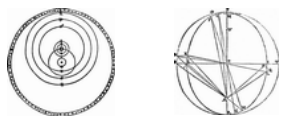
\includegraphics[width=\columnwidth]{examplefigure.png}
\caption{\label{fig:X}Title of the figure, left-justified, subsequent text indented. Place figures at the top or bottom of a column wherever possible, as close as possible to the first references to them in the manuscript. Restrict them to single-column width unless this would make them illegible.} 
\end{figure}

\subsection{Graph Lines, Drawings, and Tables}
Use black ink on white manuscript and position to fit within one of the columns on the page, and ensure that they remain still readable.

Tables with a moderate amount of information should be positioned within one column. Tables, graphs, or pictures with large amounts of information may extend across two columns.

\begin{table}
\begin{tabular}{rllll}
\toprule
& Venus & Earth & Mars & Jupiter \\
\midrule
$\rfrac{M}{M_E}$	& 0.82 		& 1 		& 0.11 		& 317.89	\\
$e$					& 0.007		& 0.017		& 0.093		& 0.048		\\
$R$ (AU)			& 0.7233	& 1			& 1.524		& 5.203		\\
$i$ (deg)			& 3.40		& 0			& 1.85		& 1.30		\\
$T$ (years)			& 0.62		& 1			& 1.88		& 11.86		\\
\bottomrule
\end{tabular}
\caption{\label{table:X}Title of table, left justified, subsequent text indented. Heading centered. Do not use vertical lines within the table; use horizontal lines only to separate headings from table entries.}
\end{table}

\subsection{Captions, Graph Axes, Legends}
Captions, graph axes, legends, \textit{etc.}, should be large enough to remain legible.

\subsection{Footnotes, Symbols, and Abbreviations}
Footnotes should be cited using symbols in this order: \footnote{Footnote 1} \footnote{Footnote 2} \footnote{Footnote 3} \footnote{Footnote 4} \footnote{Footnote 5} \footnote{Footnote 6} \footnote{Footnote 7} \footnote{Footnote 8}. Use only standard symbols and abbreviations in text and illustrations.

\subsection{Page Numbers}
Indicate page numbering at the bottom of each page.


\end{document}